\section{Introduction}

Atomic chains form one of the prototypical systems in the study of
molecular electronic systems. Atomic nanowires can be fabricated on
inert surfaces \cite{segovia1999nature,nilius2002science} or in
mechanically controlled break junctions \cite{vanruitenbeek1998mcbj}.
Atomic nanowires are of fundamental scientific interest as they form
electronic one-dimensional systems and for technology they may be viewed
as the limit for metal interconnects in use for nanoelectronics.  Atomic
nanowires are also useful for benchmarking one-dimensional quantum
transport formulations as experiments for these systems provide well
defined and understood conductance values.

Some of the earliest theoretical work with explicit treatment of the
electronic within a quatum transport study of atomic chains is due to
Lang~\cite{Lang1995prb} and this work has served as the prototype for
subsequent studies in molecular tunnel junctions. In this early work,
jellium electrodes are coupled to metal atom chains and the electronic
structure of the system is treated using \ac{DFT}. The Kohn-Sham states
from \ac{DFT} are treated as quasiparticles and the Lippmann-Schwinger
scattering equations are solved for the case of an external voltage bias
applied to the electrodes. Similar scattering approaches in conjunction
with tight binding Hamiltonians applied to the conductance of molecular
junctions combined with Landauer-B\"uttiker theory for electron transport
\cite{emberlykirczenow1999standingwave,
emberlykirczenow2000molecularwire} have been undertaken. 
Subsequently, similar methods have gained prominence by combining a \ac{DFT}
treatment of the electronic structure with a formal \ac{NEGF} treatment of
transport in open systems. More recently, the {\it GW}
approximation~\cite{hedin1965gw} has been introduced to improve  the
quaisparticle description of atomic scale tunnel junctions beyond a Kohn-Sham
description~\cite{thygesen_rubio,neaton2007amines}.  Use of the
Kohn-Sham energies in the NEGF formulation implies a single determinant
approximation to the many-electron Green's function and similarly the
{\it GW} approximation may be viewed as dynamically screened version of
the Hartree-Fock theory, likewise implying a single determinant
approximation to the many-electron Green's function.  Alternative to
these methods are to use the ideas of exact diagonalization or
configuration interaction in rate equation formulations of electron
transport~\cite{pedersen_many_body_tunneling} or through a many-electron
scattering formulation of the transport problem~\cite{vici2004}. 

In defining models for atomic-scale transport junctions, a partitioning
of the system into semi-infinite electrodes and device region is usually
performed. The device region is given by an explicit model that includes
the device (i.e. atomic chain, molecule, nanowire) as well as a region
that defines the bonding of the device to electrodes, resulting in an
'extended device' or 'extended molecule' region. The portion of the
electrode not explicitly treated by the extended device region is in
most theoretical studies treated by electrode self-energies. In this
approximation, electronic excitations in the electrode region are not
considered. Exceptions to the restriction include
ref.~\cite{galperin_nitzan2006leadexcitations} where the effect of coupling
of lead excitations to a two state model of a molecular tunnel junction is
explored, or as in a recent formulation of \ac{NEGF} that allows for
electrode interactions to be explicitly treated~\cite{ness2012jpa_leadnegf}.
In the calculations in ref.~\cite{galperin_nitzan2006leadexcitations}, it is
found for certain ranges of electrode couplings and with left-right asymmetry,
that the current arising from lead excitations can be comparable to the
current flowing due to direct tunneling.

In the following, we apply the method of configuration interaction to a
simple model of electrodes coupled to atomic chain to investigate the
influence of electron correlations on quasiparticle states arising from
the device region, and in addition we consider the influence of electrode
excitations as they couple to the device region. This approach enables
us to study the junction in an uncorrelated limit (single determinant
approximation), and to systematically include electron correlations on
the device region and electrodes to study how the quasiparticle states
evolve. By allowing electrode excitations to enter the calculation, we
are able to explore how correlated electrons on the device region
interact with electrode excitations.

% In earlier work~\cite{henderson}, a method was outlined in which an
% energy-dependent self-energy is mapped to an energy-independent
% \ac{CAP}, which, when added to the Hamiltonian, can be used in a
% many-body treatment of the system. Here, we present a continuation of
% that work, applying the method to a chain of atoms with interacting
% electrons, and using a complex \ac{CI} scheme for the calculation of
% electronic structure. Different levels of correlation are studied by
% varying the threshold parameter for \acp{CSF} in the \ac{CI} calculation.
% 
% The rest of this paper is organized as follows: in
% section~\ref{sec:method}, we cover the methods used in this work, both for
% constructing the \ac{CAP} and for solving the resulting complex symmetric
% many-body problem. In section~\ref{sec:results} we present and discuss some
% results of applying the formalism to a simple atomic chain system. Finally,
% section~\ref{sec:conclusions} contains conclusions and further perspectives.

\section{Method}
\label{sec:method}

\subsection{Model System}
\label{subsec:modelsystem}

The extended device we study is built from a simple atomic chain
consisting of 68 gold atoms with an interatomic separation of 0.28 nm
corresponding to gold chains studied experimentally in
ref.~\cite{nilius2002science} (see figure~\ref{fig:chaincapdevice}).
Within the explicit chain region, two interatomic spacings are chosen
larger than all other atom spacings to define a `molecule' between two
leads. The explicit left and right leads are each composed of 24 atoms,
and the central molecular region is composed of 20 atoms. The width of
the gap between the leads and molecule determines the strength of the
coupling and varying the spacing allows the different coupling regimes
to be investigated. 

\begin{figure}
	\begin{center}
		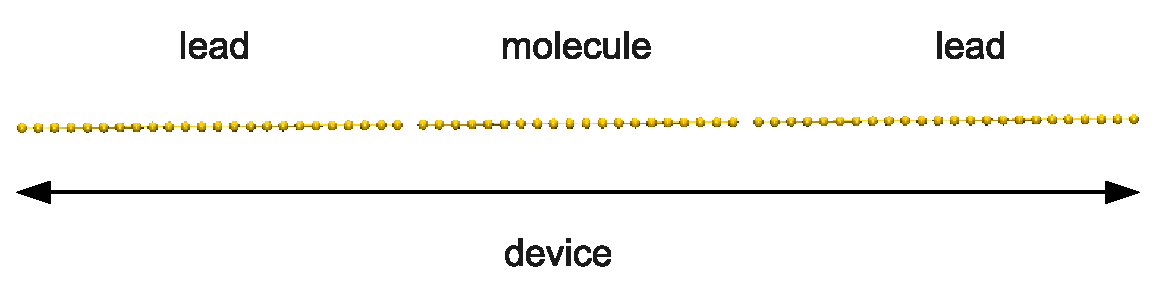
\includegraphics[width=0.9\linewidth]{figures/chaincapdevice}
	\end{center}
	\caption{Model system studied in this work. The molecule consists of
        20 Gold atoms, while the leads each consist of 24 atoms. The spacing
        between molecules and electrodes determines the coupling of the
        molecular states to the electrodes.}
	\label{fig:chaincapdevice}
\end{figure}

The regions outside of the explicit atomic region are described by a
\ac{CAP} in analogy to the use of electrode self-energies. The details of
the ab initio \ac{CAP} used are described below and its use has advantages
when including electron correlations into the calculations. In
zero$^{th}$ order, we use the Hartree-Fock approximation to calculate
quasiparticle states and the transmission spectrum for the model system
is calculated using a scattering Green's function approach as
implemented in the TIMES program~\cite{times} with the electrodes in
these calculations described using standard electrode self-energies.
This scattering calculation delivers the Hartree-Fock quasiparticle
spectrum including the energy shifts and state broadening that arise
from coupling the molecular region to electrodes, and serves as the
reference point for discussing subsequent calculations performed at
different levels of approximation.

% Isn't it a bit strange to emphasize HF as the 0th order approximation
% when we decided that the single determinant QP spectrum (with wider peaks
% than Koopmans) was not something we wanted to dwell on?

\subsection{Complex Absorbing Potential}
\label{subsec:CAP}

To treat electron correlations, we apply the method of \ac{CI}. The \ac{CI}
method is the application of the Rayleigh-Ritz linear variational principle
to the calculation of quantum many-electron energies. Within this approach,
the many-electron wavefunction is expanded in terms of Slater determinants
(or spin-coupled sums of determinants referred to as \acp{CSF}). Variation
of the \ac{CI} expansion coefficients leads to a matrix eigenvalue problem

\begin{equation}
\um{H} \vec{c} = E \um{S} \vec{c},
\end{equation} 

where $\um{H}$ is the matrix representation of the many-electron
Hamiltonian in the CSF basis, $\um{S}$ is the metric for the CSF basis,
$E$ is a many-electron energy and $\vec{c}$ is the vector of the
expansion coefficients or 'CI vector'. The matrix elements of $\um{H}$
and $\um{S}$ are constructed from one- and two-electron integrals
defined in the single particle basis used to construct the CSFs, and for
example can be Hartree-Fock states. However, in this treatment of the
many-electron problem no reference is made to single particle or
quasiparticle energies. Hence the inclusion of the electrodes into the
CI problem using electrode self-energies is complicated by the fact that
the self-energies are functions of the quasiparticle energies on the
electrodes. To avoid this complication, we employ instead energy-independent
\acp{CAP} that serve as replacement to the self-energy terms, eliminating
reference to single particle energies into the resulting \ac{CI} problem.
Note however, that by opening the system using either electrode self-energies
or \acp{CAP},  the traditionally Hermitian \ac{CI} generalized eigenvalue
problem becomes a complex symmetric generalized eigenvalue problem. The
procedure for construction of an energy-independent \ai \ac{CAP} from the
energy-dependant self-energy is discussed in detail in ref.~\cite{henderson}.
We briefly cover the essential points needed for the generation of the
\ac{CAP} in the following.

We first consider two electrodes described by known left ($\Sigma_L(\omega)$)
and right ($\Sigma_R(\omega)$) self-energies. In practice, the complex valued
self-energies for the electrodes are calculated using the TIMES
program~\cite{times}. These self-energies are added to the device region
Hamiltonian $\um{H}_D$ to yield
 
\begin{subequations}
\begin{align}
        [\um{H}_D + \lambda \um{\Sigma_L}(\omega_i^\lambda)
            +\lambda \um{\Sigma_R}(\omega_i^\lambda)] \ket{U_i^\lambda}
        &= \omega_i^\lambda \ket{U_i^\lambda} \\
        \bra{V_i^\lambda} [\um{H}_D + \lambda \um{\Sigma_L}(\omega_i^\lambda)
            +\lambda \um{\Sigma_R}(\omega_i^\lambda)]
        &= \omega_i^\lambda \bra{V_i^\lambda},
        \label{eq:adiabaticap}
\end{align}
\end{subequations}

where the parameter $\lambda$ is introduced to allow for an adiabatic
coupling between the electrode states and the extended device region
'molecular states'.  At $\lambda = 0$, the states on the extended device
region are obtained as described by eigenvectors $\ket{X_i}$ (that may
be chosen real) and real eigenvalues $\varepsilon_i$. As $\lambda$ is
increased the device region and electrode single particle states begin
to couple until at $\lambda=1$, the Hartree-Fock states for the open
system are given by the complex energies $\omega_i$, right eigenvectors
$\ket{U_i}$ and left eigenvectors $\bra{V_i}$; the left and right
eigenvectors are a consequence of introducing the complex valued
self-energies into the eigenvalue problem. The introduction of the
adiabatic coupling of the self-energies permits us to 'label' the
molecular states and to follow their evolution as the system is opened.
This allows us to use the prescription given in the following to
calculate an \ai \ac{CAP} by selecting those eigenvalues that correspond
to the uncoupled device region states. At $\lambda=1$, the real part of
$\omega_i$ gives the energy of the $i$th resonance including the shift due
to electrode coupling and the imaginary part gives the level broadening.

The goal is to build an energy-independent complex potential
$\um{W} = \um{W_L} + \um{W_R}$
such that the Hamiltonian $\um{H}_D + \um{W}$ has the same eigenvalues
as when calculated using the explict self-energies. Such a Hamiltonian is
not readily constructed as when we select the different $\omega_i$, we are
as a consequence selecting different Hamiltonians
$\um{H}_D + \um{\Sigma_L}(\omega_i) + \um{\Sigma_R}(\omega_i)$
and the biorthogonality for the left and right eigenvectors does not
necessarily hold ($<V_i|U_j> \ne \delta_{ij}$). We consider instead
constructions which yield eigenvalues that approximate the $\omega_i$  and
eigenvectors that approximate the left and right eigenvectors while
satisifying biorthogonality. Given such a set of approximate eigenvectors
we write

\begin{equation}
    \um{W} = \sum_i  \ket{U^\prime_i} \omega_i \bra{V^\prime_i} - \um{H}_D
    \label{eq:capsdefUV}
\end{equation}

which for biorthogonal $\ket{V^\prime_i}$ and $\bra{U^\prime_i}$ will give by
construction an operator $\um{H}_D + \um{W}$ with the correct eigenvalues
and approximate eigenvectors. In practice we work in the real basis of the
device region and calculate

\begin{equation}
    \um{W} = \um{S} \um{X} \um{\omega}\um{X}^\dagger - \um{H}_D
    \label{eq:capsdefX}
\end{equation}

in matrix form, with $\um{S}$ the overlap or metric for the atomic
orbital basis used to describe the device region, $\um{X}^\dagger$ and
$\um{X}$ are the matrices of the eigenvectors of device region
Hamiltonion $\um{H}_D$, and $\um{\omega}$ is the eigenvalue matrix. In
practice, as the self-energies are independent of the device region for
a properly defined 'extended device region', the \acp{CAP} are generated
on the electrodes and then transformed to the molecular orbital basis of
the device region.

% This projection introduces a small amount of inaccuracy, as will be discussed
% later.

When applying this approximation to generation of the \ac{CAP}, a
comparison can be performed against the energy level shifts and broadening
obtained from explicit calculations using the self-energy. To accomplish
this comparison, we first calculate the electron transmission through
the device region using the normal formalism of the Green's function
approach. The calculation is then repeated but in the definition of the
Green's function $G$ and spectral densities $\Lambda_{L/R}$ the
self-energy terms are replaced with the \acp{CAP} $\um{W}_{L/R}$ leading
to the following expressions:

\begin{subequations}
  \begin{align}
    G^{-1} &= [E\um{S}_0 - (\um{H}_0 + \um{W})], \\
    \Lambda_{L/R)} &= i \left( \um{W}_{L/R} - \um{W}^\dagger_{L/R)}
    \right).
  \end{align}
  \label{eq:glambdadef}
\end{subequations}

The transmission is then calculated as

\begin{equation}
  T = \um{Tr} \left[ \Lambda_L G \Lambda_R G^\dagger \right]
  \label{eq:transmfromG}
\end{equation}

whith the \acp{CAP} playing the role of the electrode self-energies.
The comparison obtained in this manner is shown in
figure~\ref{fig:transdat} revealing that the \ac{CAP} provides an
accurate energy-independent representation of the self-energies and in
particular, good agreement is achieved on the energy range around the
\ac{HOMO}-\ac{LUMO} gap of interest for subsequent investigations.

\begin{figure} 
	\begin{center}
		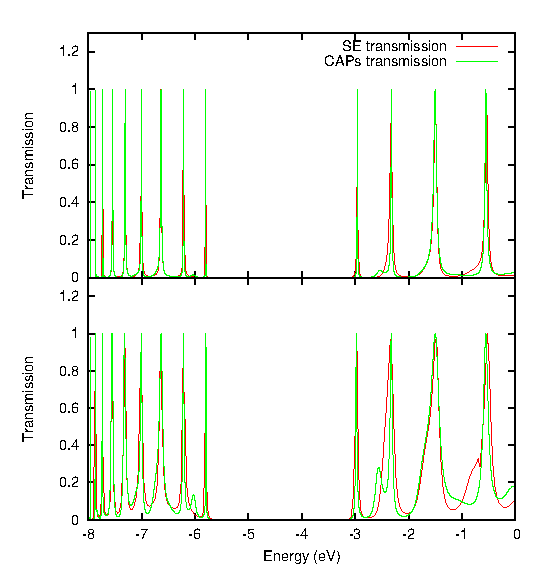
\includegraphics[width=0.9\linewidth]{figures/transdat.eps}
	\end{center}
	\caption{Transmission through the 0.45 nm (top) and 0.40 nm (bottom)
	         systems. The red curve is a transmission spectrum obtained
		 using a conventional self-energy, the green curve is obtained
		 using a \ac{CAP}.}
	\label{fig:transdat}
\end{figure}

\subsection{Complex Monte Carlo Configuration Interaction}

All \ac{CI} calculations  performed use a version of the \ac{MCCI}
program~\cite{mcci1995, mcci1998} modified to treat the complex
symmetric generalized eigenvalue problem that arises when adding the
\ac{CAP}s as a one-body operator to the many-electron Coulomb
Hamiltonian used to describe the extended device region and its
interaction with the elecrodes. \ac{MCCI} uses a Lanczos method for
matrix diagonalization and in the newest version of the program the
projection method outlined in~\cite{tarantelli_csd} is introduced to
solve the complex symmetric generalized eigenvalue problem. \ac{MCCI}
computes energy estimates by an iterative process, starting from a set
of \acp{CSF} (which initially may be a single Slater determinant).
Relative to the trial vector, additional \acp{CSF} are randomly
generated by single and double excitations relative the \acp{CSF} in the
trial vector. The \ac{CI} matrix diagonalization problem is solved on
the subspace defined by the resulting expanded vector. This vector is
then screened or 'pruned' by removing \acp{CSF} whose associated coefficient
in the \ac{CI} eigenvector has a magnitude lower than a given coefficient
threshold. This 'pruned' vector serves as trial vector for the generation of
a new set of randomly generated \acp{CSF}, and the process is repeated until
convergence is reached. Details of the \ac{MCCI} method may be found
in refs.~\cite{mcci1995,mcci1998,mcci2000,multiref}.

The use of \ac{MCCI} in the present study allows us to follow the
evolution of quasiparticle energies as electron correlations are
increased; this is achieved by starting from a single determinant picture
and then systematically including important electron correlations by
performing \ac{CI} calculations at different values of the coefficient
selection threshold. As the coefficient selection threshold is reduced,
more \acp{CSF} are included in the calculations leading to a more highly
correlated model.

\subsection{Complex Quasiparticle Energies}

From a many-electron standpoint, energy differences between
many-electron states determine quasiparticle excitations, as well as
electron affinities and ionization energies or addition and substraction
energies, respectively. In this study, we focus on the electron
affinities and ionization potentials of the {\it explicit} device
region. For example, the the electron affinity is given by the
difference in energies for the $N$-particle state $E^N$ and the
$(N+1)$-particle state $E^{N+1}$
\begin{equation}
\omega_{\rm EA} = E^{N+1} -E^N
\end{equation}
and similarly the ionization potential
\begin{equation}
\omega_{\rm IP} =  E^N - E^{N-1}
\end{equation}
is the energy difference between the $N-1$ and $N$ many-electron states.
Through the introduction of \acp{CAP}, the device region becomes an open
system resulting in complex many-electron energies. Hence the
quasiparticles energies $\omega$ are complex. It is the real energy
shift and imaginary lifetime due to the opening of the system as well
as due to the introduction of electron correlations which we study for
the molecular device states.
From the transmission calculations on our model using a scattering Green's
function approach, the transmission of the states that evolve from the
uncoupled device states is determined. It is found that these states have
transmission values close to unity and their lineshapes can be roughly
approximated by a Lorentzian profile (there is some indication of Fano-type
resonances indicating that there is a degree of coupling between left and
right electrodes, but these effects are small and do not influence our
results). Thus in order to compare to transmission spectra obtained from the
single-particle scattering Green's function calculations picture, we construct
Lorentzian peaks from the complex quasiparticles $\omega_i$:
\begin{equation}
        f(\varepsilon;\omega_i)
        = \frac{\left( \Gamma/2 \right)^2}
               {(\varepsilon - \operatorname{Re}(\omega_i))^2
               + \left( \Gamma/2 \right)^2}
        \label{eq:lobro}
\end{equation}
where $\Gamma = 2 \operatorname{Im}(\omega_i)$ is the lifetime of the
quasiparticle (i.e. the width of the Lorentzian peak).

\section{Results and Discussion}
\label{sec:results}

\subsection{Single-Particle Picture}
\label{subsec:SingleParticle}

As a validation of the \ac{CAP} approach, we would first like to see whether
the \ac{CAP} as generated according to the description of
section~\ref{subsec:CAP} gives the correct complex single-particle eigenvalues,
i.e. whether the selected self-consistent solutions of the Dyson
equations~\ref{eq:adiabaticap} provide an accurate picture of the resonances
in the device region. To do this, we construct Lorentzian peaks from the
eigenvalues, and compare to a transmission spectrum of the device obtained
using the self-energy in the \ac{NEGF} formalism. Such a comparison is shown in
figure~\ref{fig:13evals}.

This is a case of weak coupling, as can be seen by the narrowness of the
transmission peaks, and by the fact that they are not significantly shifted
from the real-valued Hartree-Fock single-particle levels. The agreement between
the Green function transmission (red) and the peaks derived from the
eigenvalues of $\um{H}_0 + \um{W}$ (green) is excellent, both in terms of
position (real part) and width (imaginary part). In the inset, the region
around the \ac{HOMO} is plotted in detail, showing the extent of the agreement
between the two methods (the green and red curves practically overlap).

\begin{figure} 
	\begin{center}
		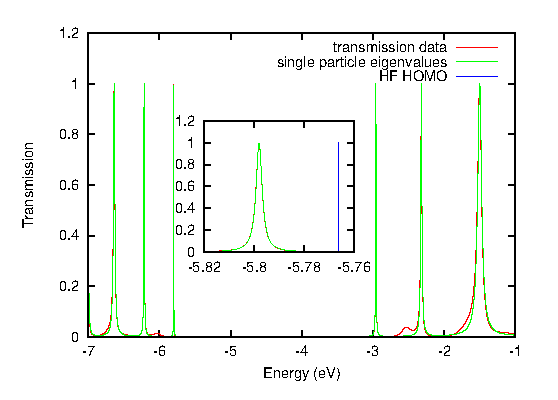
\includegraphics[width=0.9\linewidth]{figures/13evals}
	\end{center}
	\caption{Comparison of transmission data (red) with Lorentzian
	broadened complex eigenvalues of $\um{H}_0 + \um{W}$ (green) for a
	model system as described in section~\ref{subsec:modelsystem}, with
	device-lead gap of 0.45 nm. Transmission data was obtained from
	\ac{NEGF} calculations with the TIMES program~\cite{times}.
	The inset shows a close-up view of the \ac{HOMO}, with the HF \ac{HOMO}
	shown in blue for reference.
	}
	\label{fig:13evals}
\end{figure}

\subsection{Single Determinant}
\label{subsec:SingleDeterminant}

The next step is to pass to the many-body picture, initially representing the
many-body wave function of the system as a single Slater determinant. The
quasiparticle peaks in the transmission spectrum are approximated by taking
differences of many-body energies: $E^N - E^{N-1}$ yields the \ac{HOMO}, while
likewise $E^{N+1} - E^N$ yields the \ac{LUMO} (other quasiparticle levels can be
obtained by taking differences of excited many-body energies). The peaks for
the \ac{HOMO} and \ac{LUMO} of the system obtained in this way are plotted in
figures~\ref{fig:nobranch45A} and \ref{fig:nobranch40A}. There is good
correspondence in the position of the peaks, but the single determinant
difference peaks are significantly broader than their transmission spectrum
counterparts. The only difference with the single-particle eigenvalue picture
previously shown is that now, as mentioned earlier, we have projected the
eigenvectors into the $\um{X}$ basis (eigenbasis of $\um{H}_0$) instead of
representing them in their natural basis $\um{U}$ (left eigenbasis of
$\um{H}_0 + \um{W}$).
% The reason for this is that our \ac{CI} code is constrained to work with a real
% basis of MOs.

\begin{figure}[h]
	\begin{center}
		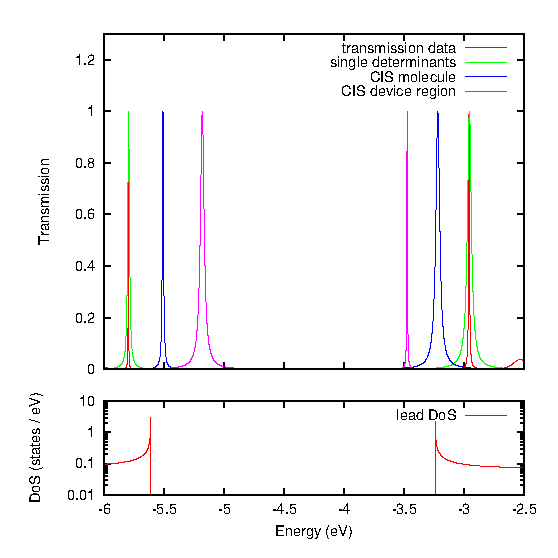
\includegraphics[width=0.9\linewidth]{figures/nobrsingles45A.eps}
	\end{center}
	\caption{4.5A system: Comparison of the transmission from Green
                 functions (red) to the Lorentzian peaks obtained by
                 subtracting single-determinant many-body energies (green).}
	\label{fig:nobranch45A}
\end{figure}

\begin{figure}[h]
	\begin{center}
		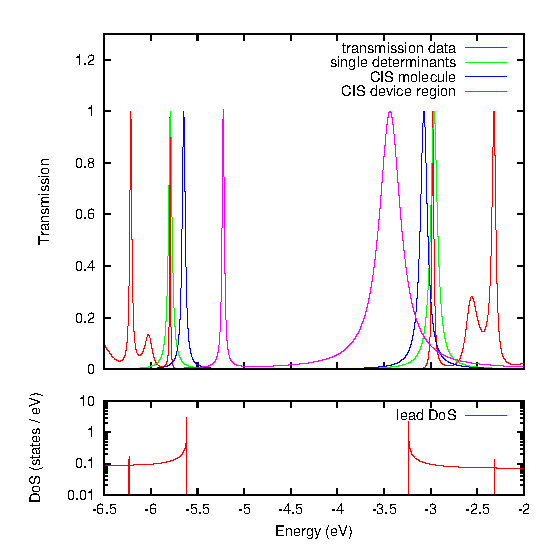
\includegraphics[width=0.9\linewidth]{figures/nobrsingles40A.eps}
	\end{center}
	\caption{4.0A system: Comparison of the transmission from Green
                 functions (red) to the Lorentzian peaks obtained by
                 subtracting single-determinant many-body energies (green).}
	\label{fig:nobranch40A}
\end{figure}

\subsection{Single Excitations}
\label{subsec:singles}

The next step is to include, for each state, the reference determinant plus all
its single excitations. By Thouless' theorem~\cite{Thouless}, to first order in
the coefficients of the non-reference \acp{CSF}, the wave function obtained by
diagonalizing in this space would still be describable as a single determinant
(and thus, by definition, contain no correlation), but by adding degrees of
freedom to the system, a degree of self-consistency is attained. This is similar
to a $\Delta$-SCF calculation, where many-body energies of different particle
number are compared at the SCF level.

We make a distinction between two types of ``singles'' \ac{CI} vectors: for the
``molecule'' calculations, the \ac{CI} space was truncated to contain only
excitations from and to MOs of the molecule (this set was found by comparing
the real parts of the complex eigenvalues $\omega_i$ with the positions of the
peaks of the respective transmission spectrum). The ``device region''
calculations contain the full singles \ac{CI} vector, i.e. all single
excitations plus the reference determinant. The results are plotted in
figures~\ref{fig:nobranch45A} and \ref{fig:nobranch40A}.

At this point, it is useful to compare the error in the two cases discussed
thus far. To relate the many-body energies to the single-particle levels, we
start by considering the following equation for the total energy of the system
(which we assume to be closed-shell) in terms of complex single-particle
energies

\begin{equation}
	E = \sum_i \omega_i - \frac{1}{2} \sum_{i,j} g_{ij}
	\label{eq:sptotalenergy}
\end{equation}

which reflects the fact that when summing the single particle energies, the
two-body terms are counted twice and must be subtracted out to obtain the total
energy. On the other hand, from the many-body point of view, we have

\begin{equation}
	E_{mb} = \sum_i h_i + \frac{1}{2} \sum_{i,j} g_{ij}.
	\label{eq:mbtotalenergy}
\end{equation}

It follows that

\begin{equation}
	\sum_i \omega_i = E_{mb} + \frac{1}{2} \sum_{i,j} g_{ij}.
	\label{eq:eesumcomparison}
\end{equation}

In other words, we can compare the obtained many body energies in both the
single determinant and single excitations cases, and determine whether the
additional degrees of freedom are able to compensate the error inherent in the
basis conversion. Such comparisons are meaningful since the single excitations
vector contains no correlation energy, but that would not be the case in a more
extensive \ac{CI} scheme. Table \ref{tab:eesum} contains the comparisons for
the 0.45 nm system with 68 electrons.

% FULL PRECISION VALUES
%               & single determinant & single excitations & $\sum \omega_i$ \\
%   real part      & -17.978662182501026 & -17.979628470130947 & -17.978417894\\
%   imaginary part & -0.12546017404575291 & -0.1252335053564404 & -0.1252903752532\\
\begin{table}
  \centering
  \begin{tabular}{l r r r} 
    \hline
                 & single determinant & single excitations & $\sum \omega_i$ \\
    \hline
    real part      & -17.97866 & -17.97962 & -17.97841\\
    imaginary part & -0.12546 & -0.12523 & -0.12529\\
    \hline
  \end{tabular}
  \caption{Comparison of many-body energies (columns 1 and 2) with
           single-particle levels (column 3).}
  \label{tab:eesum}
\end{table}

For the single determinant case, we obtain good agreement in the real part, but
a significant error in the imaginary part, consistent with behaviour plotted in
figure~\ref{fig:nobranch45A}. Again, this is due to the real basis not being 
well able to reproduce imaginary eigenvectors. For the single excitations case,
the situation is reversed; for the real part we get an error which we ascribe
to the finite expansion (Thouless' theorem is strictly only valid in an
infinite basis), whereas for the imaginary part we get good agreement, due to
the fact that our complex \ac{CI} code was able to assign complex coefficients
to the \acp{CSF} and thus reproduce the imaginary part of the energy better.

\subsection{Complex \ac{CI}}

We now move on to the \ac{CI} results, where the criterion for inclusion of a
\ac{CSF} in the \ac{CI} vector is simply its coefficient in the wave function,
and the threshold is a program parameter which can be varied to include a given
amount of correlation. The results for both systems have been plotted together,
in figure~\ref{fig:cihomo} for the \ac{HOMO}, and figure~\ref{fig:cilumo}
for the \ac{LUMO}. The curves labeled ``unrestricted'' indicate that the \ac{CI}
procedure was not limited to MOs on the molecule; MOs localized on the lead
sections of the device were also included. Note that in this case, the QP gap
widens as compared to the HF case, which would seem to be in contrast to
earlier findings which indicated that screening effects on the metal leads
renormalize the levels of the device, leading to lower
gaps~\cite{thygesen_rubio, thygesen}. This behaviour persists however, in
\ac{CI} calculations performed on the system in absence of a \acp{CAP},
indicating that this is a physical effect.

As can be seen in the figures, the \ac{CI} gap is slightly smaller than the HF
gap, and decreases with increasing correlation, consistent with the HF and GW
results in~\cite{thygesen_rubio, thygesenrubio2010corr}. In both cases the peak
widths are larger than the corresponding transmssion (HF) peaks, but similar
to the single excitations peaks, indicating that the broadening is accurately
captured at the level of single excitations.

\begin{figure}
	\begin{center}
		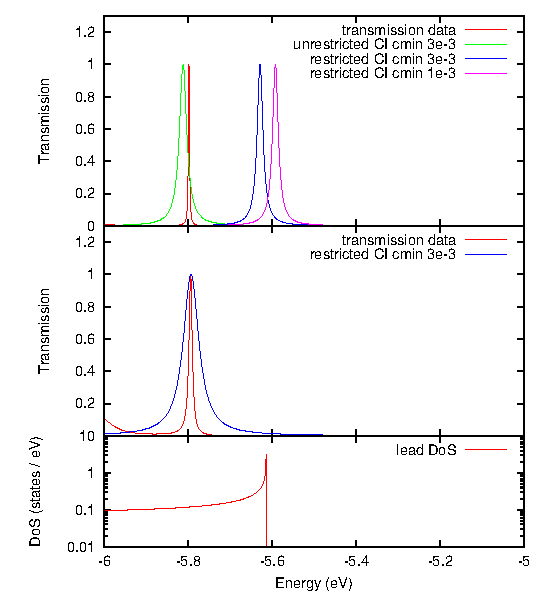
\includegraphics[width=0.9\linewidth]{figures/cihomo.eps}
	\end{center}
	\caption{CI for the \ac{HOMO} of the 0.45 (top) and 0.40 nm (middle)
                 systems, with the Density of States of the leads plotted
                 below.}
	\label{fig:cihomo}
\end{figure}


\begin{figure}
	\begin{center}
		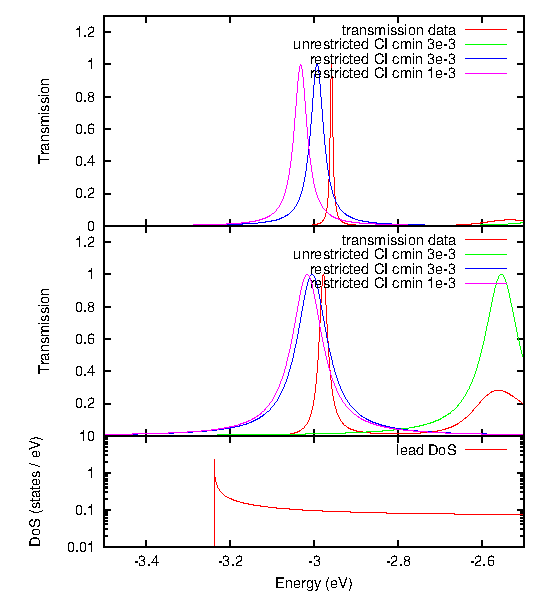
\includegraphics[width=0.9\linewidth]{figures/cilumo.eps}
	\end{center}
	\caption{CI for the \ac{LUMO} of the 0.45 (top) and 0.40 nm (middle)
                 systems, with the Density of States of the leads plotted
                 below.}
	\label{fig:cilumo}
\end{figure}

\section{Conclusions}
\label{sec:conclusions}

In this work we presented what to our knowledge are the first application
of wavefunction methods to the study of semi-infinite systems using acomplex
absorbing potential. For different degrees of molecule-lead coupling and
different levels of correlation, the complex quasiparticle peaks of a system
consisting of atomic gold chains were evaluated.

The ability to accurately describe these levels (which in this case
correspond to \ac{IP} and \ac{EA}) has been shown to be closely related to an
accurate description of transport~\cite{golden}. This work opens the door for
the application of non-empirical wave funcion methods to the study of quantum
transport in nanoscale systems in which the lifetime broadening is captured
accurately by a self-energy-derived \ac{CAP}.
